\documentclass[dvipdfmx,autodetect-engine]{ujarticle}
% 環境設定 -> 設定プロファイル -> upTex(ptex2pdf)
\setlength{\topmargin}{-45pt}
\setlength{\oddsidemargin}{-7.5mm}
\setlength{\textheight}{24.1cm}
\setlength{\textwidth}{17.4cm}
\setlength{\columnsep}{11mm}

\kanjiskip=.07zw plus.5pt minus.5pt

\usepackage[dvipdfmx]{graphicx}
\usepackage{bm}
\usepackage{url}
\usepackage[subrefformat=parens]{subcaption}
\captionsetup{compatibility=false}
\usepackage{amsmath}
\usepackage{amsfonts}
\usepackage{nidanfloat}
\usepackage{colortbl}
\usepackage{booktabs}
\usepackage{multirow}
\usepackage{algorithm}
\usepackage{algorithmic}
\usepackage{color}
\usepackage{subcaption}

\begin{document}

\twocolumn[
\noindent
\hspace{1em}
%日付
2020 年 8 月 12 日 (水)  進化型計算特論最終レポート
\hfill
M1, 2200104007 飯倉 陸
\vspace{2mm}
\hrule
\begin{center}
	{\Large \bf TDGA における 2 遺伝子座ごとのエントロピー評価に関する一考察}
\end{center}
\hrule
\vspace{3mm}
]

\section{概要}
本稿では,森ら \cite{199682} が提案した GA における選択プロセスに熱力学的なエントロピーと温度の概念を導入した熱力学的遺伝アルゴリズム (Thermodynamical Genetic Algorithm: TDGA) の機能拡張に関する考察を述べる.
具体的には,TDGA 特有の問題である TDGA 収束に対するアプローチとして森らが指摘した,エントロピーを 2 遺伝子座ごとに評価する手法について検討する.

\section{実装上の変更点}
実装上は,エントロピーを計算する際の個体表現を変更した.
具体的には,対立遺伝子を 2 値 $\{0, 1\}$ とした場合に隣接する 2 つの遺伝子座の遺伝子を 2 進数表現として捉え,10 進数表現に変換した.
これによって,対立遺伝子は 4 値 $\{0, 1, 2, 3\}$ となる.
また,変換前の遺伝子長を $M$ とすると,変換後の遺伝子長は $M-1$ となることに注意する.
例えば以下のように,個体 $x_{1}$ は $x_{1}'$ に変換される.
	\begin{equation}
		x_{1} : 1 0 1 1 0 0 1 0 \notag
	\end{equation}
	\begin{equation}
		x_{1}' : 2 1 3 2 0 1 2   \notag
	\end{equation}
この変更に伴い,エントロピーの計算式は以下のようになる.
	\begin{equation}
		H^{2} = \sum^{M-1}_{k=1} H^{2}_{k}, H^{2}_{k} = - \sum_{j \in \{0,1,2,3\}} P_{j}^{k} \log P_{j}^{k}
	\end{equation}
ここで,$H^{2}$ は 2 遺伝子座ごとに計算したエントロピーを表し,$M$ は対立遺伝子を 2 値 $\{0, 1\}$ とした場合の遺伝子長である.
また, $H_{k}^{2}$ は個体群の遺伝子座 $k$ の遺伝子に関するエントロピーを,$P_{j}^{k}$ は遺伝子座 $k$ における対立遺伝子 $j$ の存在確率を表している.

\section{評価実験}
本章では,エントロピーを 2 遺伝子座ごとに評価した TDGA を,シミュレーションによって従来の TDGA および SGA と比較することにより,その有効性について検討する.

	\subsection{実験条件}
	シミュレーションの条件については森ら \cite{199682} に従い,表 1 に示す 30 荷物のナップサック問題を扱う.
	\begin{table*}[t]
		\begin{center}
			\caption{30 荷物ナップサック問題詳細 (\cite{199682} より引用)}
			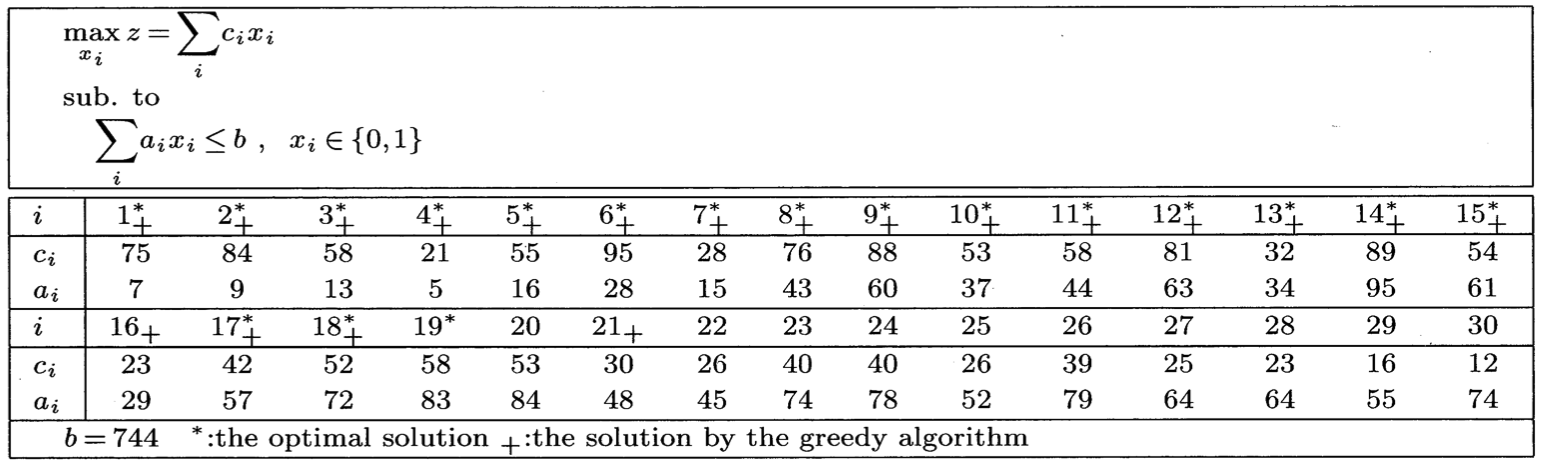
\includegraphics[width=15cm]{./fig/knapsack.png}
			\label{fig:knapsack}
		\end{center}
	\end{table*}
	具体的には各アルゴリズムについて突然変異率および個体数を変え,30 回問題を解かせた場合に 100 世代以内に最適解を獲得した回数を調べる.
	異なる突然変異率を設定する場合,個体数として TDGA では 32,SGA では 64 を与えた.
	この実験においてそれぞれのアルゴリズムに対して最も多く最適解を得たときの突然変異率を,個体数を変化させた場合の突然変異率として設定する.
	また,いずれの場合も初期温度 $T = 10$ で設定した.

	\subsection{結果と考察}
	\begin{figure*}[htbp]
	  \begin{center}
	    \begin{tabular}{c}

	      \begin{minipage}{0.50\hsize}
	        \begin{center}
						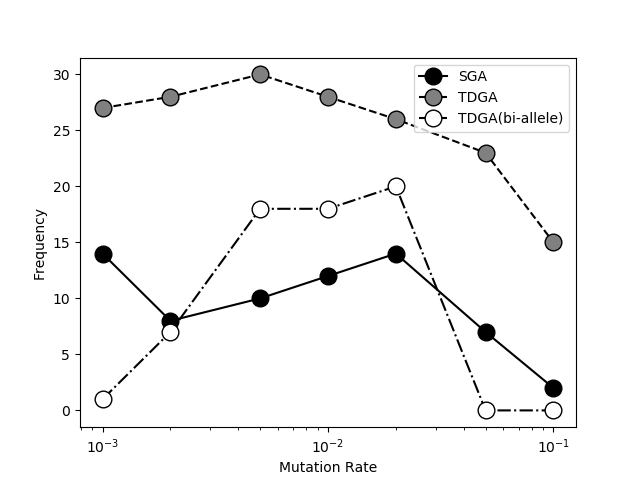
\includegraphics[width=8.5cm]{./fig/mutation_rate.png}
						\caption{突然変異率の比較}
						\label{fig:mutation_rate}
	        \end{center}
	      \end{minipage}

	      \begin{minipage}{0.50\hsize}
	        \begin{center}
						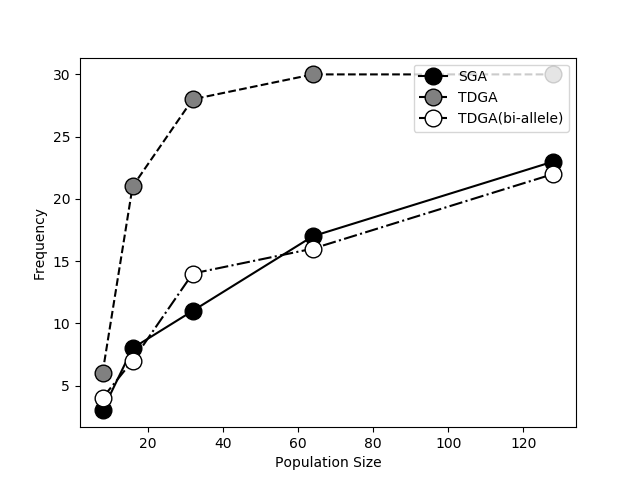
\includegraphics[width=8.5cm]{./fig/population_size.png}
						\caption{個体数の比較}
						\label{fig:population_size}
	        \end{center}
	      \end{minipage}

	    \end{tabular}
	  \end{center}
	\end{figure*}

	まず,図 1 に異なる突然変異率を設定した場合に各アルゴリズムが最適解を得た回数の比較を示す.
	図 1 から,2 遺伝子座ごとにエントロピーを計算する場合 (TDGA (bi-allele)) は,1 遺伝子座ごとにエントロピーを計算する場合 (TDGA) よりも最適解が得られる回数が少ないことがわかる.
	\par

	次に,図 2 に異なる個体数を設定した場合の各アルゴリズムが最適解を得た回数の比較を示す.
	ここでそれぞれのアルゴリズムに対して使用した突然変異率は,TDGA では 0.005,TDGA (bi-allele) では 0.02,SGA では 0.02 である.
	図 2 からわかる通り,異なる個体数を設定した場合でも,TDGA (bi-allele) は TDGA の最適解獲得回数を下回った.
	\par

	図 3 〜図 4 に各アルゴリズムを用いた場合の解の探索過程について示す.
	図 3 と図 4 を比較すると,2 遺伝子座ごとにエントロピーを評価する方が,1 遺伝子座ごとに評価するよりも目的関数値の最高値が最適解に到るまでに要する世代数が多いことがわかる.\par

	また,図 5 〜図 6 に各アルゴリズムを用いた場合の各遺伝子座におけるエントロピーを示す.
	これらは個体群の多様性を維持する様子を表現した図である.
	図 5 と図 6 を比較すると,2 遺伝子座ごとにエントロピーを評価する方が,1 遺伝子座ごとに評価するよりも全体的にエントロピーが高いことが確認できる.\par

	以上のことから,2 遺伝子座ごとにエントロピーを評価することで,より個体群の多様性を維持するようになることが考察される.
	そして今回対象とした問題では,その性質が解の探索を必要以上に複雑にし,結果として最適解を獲得する可能性を減少させたと考えられる.

	\begin{figure*}[htbp]
	  \begin{center}
	    \begin{tabular}{c}

	      \begin{minipage}{0.50\hsize}
	        \begin{center}
						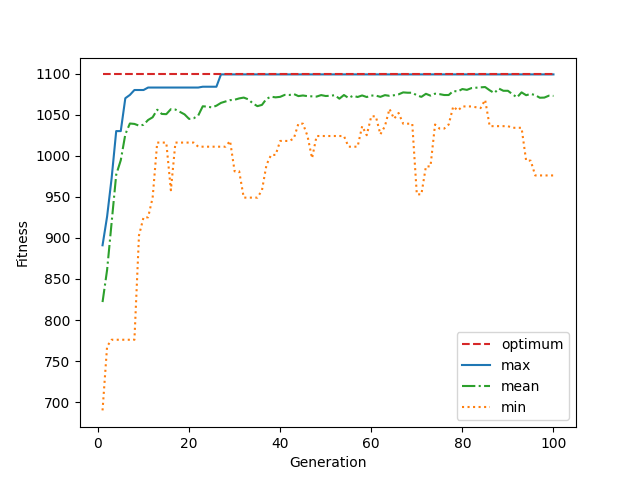
\includegraphics[width=9cm]{./fig/tdga_stats.png}
						\caption{TDGA を用いた場合の解の探索過程}
						\label{fig:tdga_stats}
	        \end{center}
	      \end{minipage}

	      \begin{minipage}{0.50\hsize}
	        \begin{center}
						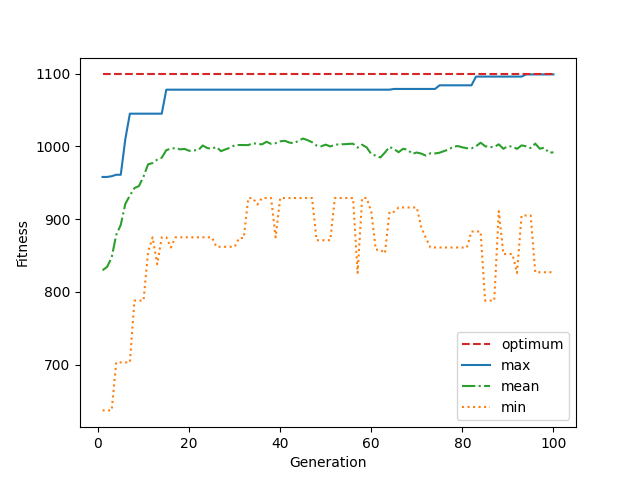
\includegraphics[width=9cm]{./fig/tdga_2_stats.png}
						\caption{TDGA (bi-allele) を用いた場合の解の探索過程}
						\label{fig:tdga_2_stats}
	        \end{center}
	      \end{minipage}

	    \end{tabular}
	  \end{center}
	\end{figure*}

	\begin{figure*}[htbp]
	  \begin{center}
	    \begin{tabular}{c}

	      \begin{minipage}{0.50\hsize}
	        \begin{center}
						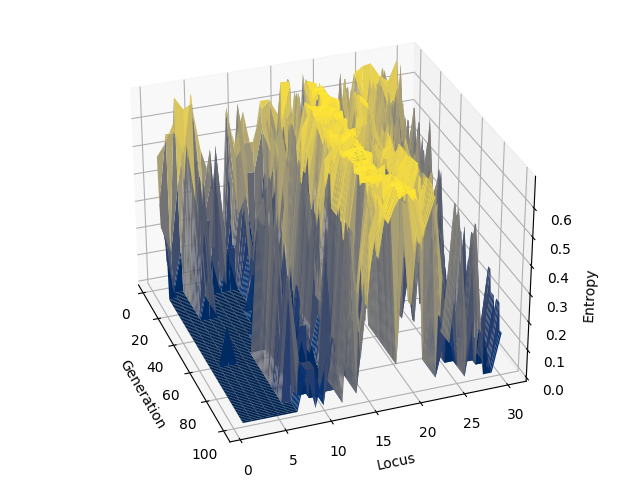
\includegraphics[width=9cm]{./fig/tdga_entropy.png}
						\caption{各遺伝子座におけるエントロピー (TDGA)}
						\label{fig:tdga_entropy}
	        \end{center}
	      \end{minipage}

	      \begin{minipage}{0.50\hsize}
	        \begin{center}
						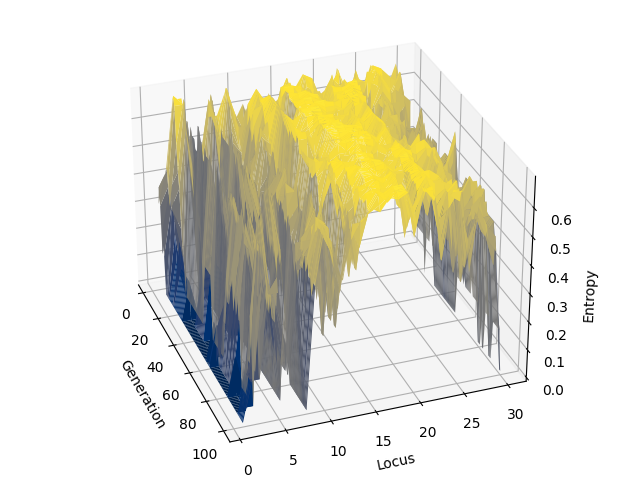
\includegraphics[width=9cm]{./fig/tdga_2_entropy.png}
						\caption{各遺伝子座におけるエントロピー (TDGA (bi-allele))}
						\label{fig:tdga_2_entropy}
	        \end{center}
	      \end{minipage}

	    \end{tabular}
	  \end{center}
	\end{figure*}

\section{おわりに}
本稿では,TDGA 収束の対策として挙げられた 2 遺伝子座ごとにエントロピーを計算することの有効性について検討した.
30 荷物ナップサック問題を対象としたシミュレーションの結果,2 遺伝子座ごとにエントロピーを計算する手法は,従来の 1 遺伝子座ごとにエントロピーを計算する手法よりも低い性能を示した.
このことから,この問題に対しては 1 遺伝子座ごとにエントロピーを評価する方が適切であるといえる.
実験において,従来の TDGA が 30 回すべての試行において最適解を獲得する場合も確認されたことから,今回扱った問題では TDGA 収束は起こりにくいことも考えられる.
そのため,TDGA 収束が発生しやすい問題を対象として解かせた場合に,2 遺伝子座ごとにエントロピーを評価することの妥当性について,今後検討する必要がある.

% 参考文献リスト
\bibliographystyle{unsrt}
\bibliography{final_report}

\end{document}
